\chapter{Theory}


\section{Standard Model}
    
    The Standard Model of particle physics has proven excellent at describing particle interactions up to the energy scale of modern colliders ($\sim$ TeV) and with the discovery of a Standard Model like Higgs Boson at the LHC the theory will be able to claim completeness up to the energy scale of modern colliders. However the Standard Model is known to be incomplete, with observations such as neutrino mass, the lack of anti-matter in the observable universe and the lack of a quantum gravity description with the related hierarchy problem (drastic difference in force strength between gravity and the other fundamental forces seen in the standard model),  the Standard Model is far from a theory of Everything. This then leaves the possibility of new physics appearing in the energy scope of the LHC.
    % talk about particles in the standard model and proton constituents.
    % maybe history of finding composite particles.


\section{Non-resonant new Physics}

    Beyond the Standard Model (BSM) or new physics models is a staple of the physics programs of the LHC detectors. Any theoretical models not contained within the Standard Model (SM) can fall in to this category and LHC experiments aim to search for as many of these models as are feasible within scope (Proton-Proton collisions and within the energy range of the LHC). Within the detection channel of two lepton decays (di-lepton), one evidence of new physics is non-resonant signals. This physics would show as a divergence from the SM prediction in the di-lepton mass spectrum unlike the resonant signals of particles such as the Z boson particle which shows as a peak in the di-lepton mass spectrum.

    Non-resonant signals could be the results of many BSM theoretical models but two main theory’s are presented here and their searches compose the rest of this thesis.


    \subsection{Contact Interaction Theory}

        The Standard Model (SM) assumes quarks and leptons to be fundamental particles in nature. This assumption is not without compelling argument but like the proton beforehand there is no reason quarks and leptons should not be composite structures or bound states of more fundamental particles, often referred to as Preons \cite{Eichten:1983hw}, at an energy scale $\Lambda$ we have yet to reach. 

        One way quark-lepton compositness would exhibit itself is in 4-fermion contact interactions between two quarks from the incoming protons producing two final state leptons ($q\bar{q} \rightarrow \ell^{-}\ell^{+}$). This is the compositness signal searched for at the ATLAS detector and as can be seen the the Faynman diagrams in Fig. \ref{fig:fd} compared to DY from which it is almost indistinguishable.

        \begin{figure}[h]
            \begin{center}
            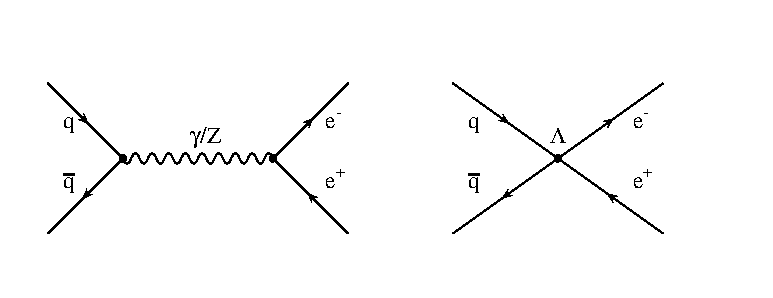
\includegraphics[scale=0.6]{images/compositeness.eps}
            \end{center}
            \caption{Feynman diagrams of a contact interaction (right) and the predominant background Drell-Yan production (left).}
            \label{fig:fd}
        \end{figure}

        Without knowing the intermediate process one can write a Lagrangian describing the new interaction; 

        \begin{equation}
            \mathcal{L} = \frac{g^{2}}{2\Lambda^{2}}
                [\eta_{LL} (\bar{\psi_{L}}\gamma_{\mu}\psi_{L}) (\bar{\psi_{L}}\gamma^{\mu}\psi_{L}) 
                + \eta_{RR} (\bar{\psi_{R}}\gamma_{\mu}\psi_{R}) (\bar{\psi_{R}}\gamma^{\mu}\psi_{R}) 
                + 2\eta_{LR} (\bar{\psi_{L}}\gamma_{\mu}\psi_{L}) (\bar{\psi_{R}}\gamma^{\mu}\psi_{R}) ]
        \end{equation}

        where $g$ is the coupling constant, $\Lambda$ is the energy scale of new physics and $\psi_{L}$ and $\psi_{R}$ are the left and right handed fermionic fields respectively. The sign of $\eta$ defines whether the new interaction interferes constructively ($\eta = -1$) or destructively ($\eta = +1$) with DY and is always unity. For previous analyses \cite{PhysRevLett.103.191803,PhysRevLett.96.211801,PhysRevD.87.015010} a benchmark model of just the Left-Left (LL) component has been used and defined by $\eta_{LL} = \pm~1$ and $\eta_{RR} = \eta_{LR} = 0$. Here however an investigation of each of the three parameters is done individually. Both the LL and RR cases are expected to behave similarly however the LR case exhibits a different angular dependence than either of the other formalisms or the DY background. This difference is the primary reason for the inclusion of the angular part of this analysis found later. The discriminating variables used are therefore dilepton invariant mass and cosine of the decay angle $\theta^{*}$. The angle $\theta^{*}$ is defined in the Collins-Soper frame \cite{PhysRevD.16.2219} which is defined with the $x$-axis perpendicular to the incoming parton momentum frame and the $z$-axis bisecting the angle between the two incoming parton momenta. Since the incoming parton information is understandably unavailable the $z$-axis is taken as the direction of the incoming quark (as opposed to anti-quark) obtained from the boost in to the dilepton frame. The angle $\theta^{*}$ is then defined as the angle between this $z$-axis the momentum of the outgoing negatively charged lepton (or electron in this analysis).

        Figure \ref{fig:theoryAFB} shows the difference expected between the LR CI models and DY background from a truth Monte-Carlo study. The variables used are $A_{FB}$ and dilepton invariant mass where $A_{FB}$ is the forward-backwards asymmetry defined in relation to cos$\theta^{*}$ as;

        \begin{equation}
            A_{FB} = 
                \frac{N_{F} - N_{B}}{N_{F} + N_{B}}
            \label{eq:AFB}
        \end{equation}

        where $N_{F}$ and $N_{B}$ are number of events found with cos$\theta^{*}$ greater than 0 and less than 0 respectively.
        
        \begin{figure}[h]
            \begin{center}
            %\includegraphics[scale=0.3]{}
            \end{center}
            \caption{MC truth level comparison between the forward backwards asymmetry of DY and and of a CI LR signal.}
            \label{fig:theoryAFB}
        \end{figure}

        A differential cross section for this interaction, $q\bar{q} \rightarrow \ell^{-}\ell^{+}$ ($qq\ell\ell$), is given by

        \begin{equation}
            \frac{d\sigma}{dm_{\ell\ell}} = 
                \frac{d\sigma_{DY}}{dm_{\ell\ell}} 
                - \eta\frac{F_{I}}{\Lambda^{2}} 
                + \frac{F_{C}}{\Lambda^{4}},
            \label{eq:DiffCross}
        \end{equation}

        where $m_{\ell\ell}$ is the dilepton mass and $\Lambda$ is the scale of the new physics. In the case of quark/lepton compositness $\Lambda$ refers to the point at which fermions stop being bound as SM quarks and leptons. $F_{I}$ and $F_{C}$ define the interference DY-CI term and the pure CI term respectively. The scale of the interference and pure term vary with both the dilepton invariant mass as well as the scale of new physics $\Lambda$.

        Experimentally this interaction would be seen as a deviation from the Standard Model (SM) Drell-Yan (DY)($q\bar{q}~\rightarrow~\gamma/Z~\rightarrow~\ell^{+}\ell^{-}$) dilepton mass spectrum as seen in Fig. \ref{fig:theoryInvMass}). 

        \begin{figure}[h]
            \begin{center}
            %\includegraphics[scale=0.3]{}
            \end{center}
            \caption{MC truth level comparison between DY spectrum with and without CI signal.}
            \label{fig:theoryInvMass}
        \end{figure}

    

    \subsection{ADD Theory}
        The large extra spacial dimensions theory described by Arkani-Hamed, Dimopoulos, and Dvali (or ADD theory) \cite{ArkaniHamed:1998rs} predicts a Graviton producing a non-resonant excess in the dilepton mass spectrum. The ADD theory describes a graviton that propagates the extra dimensions and acquires closely backed Kaluza-Klein (KK) modes that show as a broad excess above the SM background. 
        The ADD model was originally proposed to solve the hierarchy problem and bring the energy scale associated with gravity (the Planck scale M$_{Pl}$ ~ $10^{16}$ TeV) down to the level of electroweak energy scale (M$_{EM}$~ $10^{-1}$). This is achieved with the introduction of $n$ additional compactified spacial dimensions with radius $R$. This then gives a new scale in the 4+$n$ dimensional space, M$_{D}$, which is related to the Planck scale by M$_{Pl}$ = M$_{D}^{n+2}R^{n}$. If both the radius of the extra dimensions $R$ and and number $n$ are large enough this solves the hierarchy problem by bringing M$_{D}$ down to the level of M$_{EM}$.
        The Graviton is the only propagator in these extra $n$ dimensions with each dimension resulting in a new KK mass splitting of the mass peak. The mass splitting occurs with an interval of $1/R$ and since $R$ is required to be large by the theory this pushes the mass splitting together causing a continuous peak like structure analogous to a non-resonant excess. This sum over these virtual KK modes has to be regularised by an ``ultra violet'' cutoff ($\Lambda_{T}$) and it is convention to equate this cutoff to the onset of Quantum Gravity (M$_{S}$) only bellow which the theory is valid. This scale M$_{S}$ is used as the scale of physics for the ADD theory which is a low energy effective theory bellow this scale. This scale can be related to the new $n$ dimensional Planck scale (M$_{D}$) by;

        \begin{equation}
            M_{S} = 2~\sqrt{\pi}\left[{\Gamma (n/2)}\right]^{1/(n+2)}M_{D}
            \label{eq:gravScale}
        \end{equation}

        where $\Gamma$ is the decay width. Bellow the scale M$_{S}$ virtual Graviton exchange would lead to a broad excess over the SM Drell-Yan dileption mass spectrum. 
        The total differential cross-section for the dilepton SM DY and virtual Graviton exchange is then;

        \begin{equation}
            \frac{d\sigma}{dm_{\ell\ell}} =
                \frac{d\sigma_{DY}}{dm_{\ell\ell}} +
                \mathcal{F}\frac{F_{I}}{M_{S}^{4}} +
                \mathcal{F}^{2}\frac{F_{G}}{M_{S}^{8}}
            \label{eq:ADDcs}
        \end{equation}

        where $\sigma_{DY}$ is the SM DY cross-section, $F_{I}$ and $F_{G}$ are the Graviton-DY interactions term and pure virtual Graviton exchange term respectively while $\mathcal{F}$ is a formalism dependent parameter and also dimensionless. 
        Three formalisms are commonly used to describe ADD theory, these are Giudice, Rattazzi, and Wells (GRW) \cite{Giudice:1998ck}, Han, Lykken, and Zhang (HLZ) \cite{PhysRevD.59.105006} and Hewett \cite{PhysRevLett.82.4765}. Defining $\mathcal{F}$ these formalisms alter the cross-section of virtual Graviton exchange with HLZ depending on the number of extra dimensions, $n$, introduced by the ADD theory. All three formalisms are detailed in Eq. \ref{eq:ADDF}

        \begin{equation}
            \begin{aligned}
                \mathcal{F}~=&~1,   \quad &\text{(GRW)} \\
                \mathcal{F}~=&~  \left\{ 
                    \begin{array}{l l}
                        \log{(\frac{M_{S}^{2}}{m_{\ell\ell}^{2}})},      \quad & (n = 2) \\
                        \frac{2}{n-2},                                   \quad & (n > 2)
                    \end{array} \right.,  \quad &\text{(HLZ)}  \\
                \mathcal{F}~=&~\frac{2\lambda}{\pi}~=~\frac{\pm2}{\pi},     \quad &\text{(Hewett)}
            \end{aligned}
            \label{eq:ADDF}
        \end{equation}

        Of note the variable $\lambda$ found in the Hewett formalism defines the constructive or destructive nature of the gravitational interaction with the SM DY processes. $\lambda$ is always of order unity with +1 and -1 being constructive and destructive respectively.
        The GRW and HLZ with n = 2 are the two formalisms explicitly searched for in this analysis with a conversion of limits done to asses the other formalisms in the Statistical Analysis chapter.

        Experimentally this interaction would be seen as a deviation from the SM DY ($q\bar{q}~\rightarrow~\gamma/Z~\rightarrow~\ell^{-}\ell^{+}$) dilepton mass spectrum but with a cut-off where quantum gravity is assumed take effect. This can be seen in Fig. \ref{fig:theoryInvMassADD}. It is important to note that no angular difference in the virtual graviton decay is expected from that of SM DY, therefore ADD is only searched for in the dilepton mass spectrum.

        \begin{figure}[h]
            \begin{center}
            %\includegraphics[scale=0.3]{}
            \end{center}
            \caption{MC truth level comparison between DY spectrum with and without ADD signal.}
            \label{fig:theoryInvMassADD}
        \end{figure}



\section{Past Searches}

    {\bf Contact Interaction}\\
        Several previous CI analyses have been done at hadron colliders including the LHC \cite{PhysRevD.87.015010,ATLAS:2012pu,PhysRevD.87.032001,PhysRevD.87.052017} and the Tevitron \cite{PhysRevLett.103.191803,PhysRevLett.96.211801,PhysRevLett.87.231803,PhysRevLett.82.4769,PhysRevLett.79.2198}. Searches were also performed at the electron-proton collider HERA \cite{Chekanov200423,Adloff200335}, previous lepton colliders \cite{Abdallah2009.60.1,Schael2007.49.411,Abdallah2006.45.589,Abbiendi2004.33.173,Acciarri200081} and neutrino scattering experiments \cite{}. Of the results comparable to this analysis searching for $qq\ell\ell$ Contact Interactions in the absence of signal the highest limits set on the scale of new physics $\Lambda$ come from the previous ATLAS analysis \cite{PhysRevD.87.015010} detailed in appendix A. This analysis set a limit of $\Lambda$ $>$ 12.7 TeV and $\Lambda$ $>$ 9.63 TeV for the dilepton LL CI model for constructive and destructive interference respectively. The limits obtained for the electron channel for comparison to this analysis were $\Lambda$ $>$ 11.6 TeV for constructive and $\Lambda$ $>$ 8.76 TeV for destructive interference. \\


    {\bf ADD}\\
        The highest dilepton ADD limits set on the formalism normally used as a bench mark, GRW, are that of the previous ATLAS analysis \cite{PhysRevD.87.015010} discussed in Appendix A which sets a limit of 3.0 TeV on the scale of new physics (M$_{S}$). Preliminary results from CMS on the LHC data set used in this analysis do however show higher limits but are not yet published. Other previous analyses have also been carried out searching for large extra dimensions with the ADD model. These analyses have come from the LHC \cite{}, from the Tevatron \cite{}, as well as from electron-proton collider HERA \cite{} and electron-positron collider LEP \cite{}. 








